\begin{refsegment}
\chapter{GROOLS}

J'ai consacré ces trois années de recherche pour une approche interactive entre le biologiste et les prédictions bio-informatiques lors du processus de curation de l'annotation fonctionnelle des génomes bactériens. Compte tenu de l'augmentation constante et rapide des annotations automatiques, un système expert pourrait assister les biologistes à détecter les annotations inconsistantes et contradictoires. La curation et la validation des prédictions bio-informatiques pourrait alors rattraper son retard.

\section{Le début de GROOLS}

L'équipe \texttt{HELIX} d'\textit{Alain VIARI} avait commencé un projet en ce sens nommé \texttt{\gls{HERBS}} en collaboration avec le \texttt{\gls{SIB}} dans le cadre du projet \gls{HAMAP} \cite{pedruzzi2015hamap}. L'objectif de \texttt{\gls{HERBS}} était d'alerter les biologistes sur les voies métaboliques manquantes, non attendues ou encore ambiguës. Pour cela l'outil s'appuie sur un moteur d'inférence \texttt{\gls{JESS}}, d'une base de connaissance (contenant les règles et les faits, \cref{fig:systeme_expert}) et d'une interface graphique pour l'exploration des connaissances. \textit{Alain VIARI} m'a permis d'accéder l'outil PathRules qui est une implémentation de \texttt{\gls{HERBS}} avec le moteur \texttt{\gls{CLIPS}} \cite{riley1991clips} ainsi que son code source.


J'ai pris en main l'outil par l'intégration des voies de biosynthèse de la lysine (AAA et DAP) décrit par \texttt{UniPathway} et l'ajout des prédictions provenant de 79 organismes. Pour ce faire les données sont rangées dans trois dossiers présent à la racine du projet: (i) "data/processes" pour la description des voies métaboliques, (ii) "data/observers/uniprot" pour le catalogues des prédictions par espèces, (iii) "data/species" pour la description taxonomique des espèces. Les fichiers doivent porter l'extension \texttt{.data} et le nom du fichiers est utilisé comme identifiant pour faire le lien entre les processus, les , prédictions et les information taxonomique de l'espèce. Par exemple, j'ai utilisé l'identifiant ACIAD pour mettre en relation les informations d'\textit{Acinetobacter sp ADP1}.

\console{find data/ -name 'ACIAD.data'}{ data/observers/uniprot/ACIAD.data\par data/species/ACIAD.data }


La description des données dans ses fichiers suit la nomenclature \texttt{\gls{CLIPS}}. C'est à dire que les faits sont déclarés entre parenthèses. Les observations sont formatés comme suit: ( \texttt{source} (id \texttt{xxx}) (alias \texttt{yyy} sp:\texttt{zzz})  ) .

\console{head data/observers/uniprot/data/ACIAD.data}{
    (uniprot (id ASPARTATE-SEMIALDEHYDE-DEHYDROGENASE-RXN) (alias ACIAD0479 sp:ACIAD00423))\par
    (uniprot (id SUCCDIAMINOPIMDESUCC-RXN) (alias ACIAD0791 sp:ACIAD0070)\par
    (uniprot (id ASPARTATEKIN-RXN) (alias ACIAD1252 sp:ACIAD01133))\par
    (uniprot (id SUCCINYLDIAMINOPIMTRANS-RXN) (alias ACIAD2080 sp:ACIAD01886))\par
    (uniprot (id TETHYDPICSUCC-RXN) (alias ACIAD2599 sp:ACIAD02357))\par
    (uniprot (id DIAMINOPIMEPIM-RXN) (alias ACIAD2659 sp:ACIAD02412))\par
    (uniprot (id DIAMINOPIMDECARB-RXN) (alias ACIAD2660 sp:ACIAD02413))\par
    (uniprot (id DIHYDRODIPICSYN-RXN) (alias ACIAD3585 sp:ACIAD03222))\par
    (uniprot (id DIHYDROPICRED-RXN) (alias ACIAD3619 sp:ACIAD03252))\par
}


L'information taxonomique est également un fait. Il débute par "species" suivis de plusieurs chaîne de caractères pour renseigné de plus en plus précisément la taxonomie de l'organisme.

\console{cat data/species/ACIAD.data}{ (species lineage Bacteria Proteobacteria Gammaproteobacteria Pseudomonadales Moraxellaceae Acinetobacter Acinetobacter\_sp.\_ADP1) }

Pour représenter la structure hiérarchique des voies métaboliques, les fait sont organisés pour exprimé la notion de composition et d'équivalence. La notion de composition et utiliser pour relier les blocs réactionnelles à leurs réactions. Quant à l'équivalence elle permet de définir les chemins alternatif pour réaliser une voie métabolique. La syntaxe \texttt{\gls{CLIPS}} utilise $x -> \ldots$ pour signifier "x tel que \ldots". La partie à droite de la flèche décrit les relations en notation polonaise\footnote{Également connue sous le nom "notation pré-fixée". Par exemple, le calcul "$5 \times (2 + 3)$", s'écrit "$\times 5 (+ 2 3)$". }. Ci-dessous la voie métabolique de la biosynthèse de la lysine par la voie AAA (Acide Alpha-amino Adipique) selon \texttt{UniPathway}.

\console{cat data/processes/lysine\_AAA\_biosynthesis.data}{
;;;; --------------------------------------------------------\par
;;; HERBS (Hamap Expert Rules Based System)\par
;;;\par
;;; @file: lysine\_AAA\_biosynthesis.data\par
;;; --------------------------------------------------------\par
;;;\par
(process declare lysine\_AAA\_biosynthesis present in ALL)\par
(process define lysine\_AAA\_biosynthesis -> and UPA00033)\par
(process define UPA00033 -> or UPA00033-alt-0 UPA00033-alt-1)\par
(process define UPA00033-alt-0 -> and ULS00012 ULS00013)\par
(process define UPA00033-alt-1 -> and ULS00012 ULS00014)\par
(process define ULS00012 -> and ULS00012-alt-0)\par
(process define ULS00012-alt-0 -> and UER00028 UER00029 UER00030 UER00031 UER01027)\par
(process define ULS00013 -> or ULS00013-alt-0 ULS00013-alt-1)\par
(process define ULS00013-alt-0 -> and UER00032 UER00034)\par
(process define ULS00013-alt-1 -> and UER00033 UER00034)\par
(process define ULS00012 -> and ULS00012-alt-0)\par
(process define ULS00012-alt-0 -> and UER00028 UER00029 UER00030 UER00031 UER01027)\par
(process define ULS00014 -> or ULS00014-alt-0 ULS00014-alt-1)\par
(process define ULS00014-alt-0 -> and UER00035 UER00037 UER00038 UER00039)\par
(process define ULS00014-alt-1 -> and UER00036 UER00037 UER00038 UER00039)\par
}


Chaque processus est un fait désigné par le mot clé "process". Les voies métabolique sont préfixer du mot clé "declare" et "define" pour ces composants. Les faits constituant la voie métabolique sont hiérarchiquement organisé. Lorsque un fait et composé de plusieurs concepts on utilise le symbole "and" et "or" lorsqu'un fait possède des équivalences. Les lignes débutant par un point virgules ne sont pas interprété par  \texttt{\gls{CLIPS}}.

Ceci permet d'obtenir une évaluation de la complétion de l'annotation fonctionnelle des génomes (\cref{fig:herbs_rapport}).

\begin{shadedfigure}[H]
    \centering
    \includegraphics[width=\textwidth]{img/herbs_conclusion_report.png}
    \caption{Rapport sur la présence de la voie de biosynthèse de la lysine.}
    \label{fig:herbs_rapport}
\end{shadedfigure}

L'utilisateur à la possibilité d'explorer les voies métaboliques pour discriminer les composants manquants (\cref{fig:herbs_dag}).

\begin{landscape}
    \begin{shadedfigure}[H]
        \centering
        \includegraphics[width=\textwidth]{img/herbs_aciad_lysine_dap.png}
        \caption{Rapport sur la présence de la voie de biosynthèse de la lysine.}
        \label{fig:herbs_dag}
    \end{shadedfigure}
\end{landscape}


expliqué les ratés
inaptitude à tout programmer de manière explicite

\textbf{Ce qui suit doit/peut être déplacé en discussion.}

Toutefois la méthode utilisé reste assez flou d'un point de vue formel. La distinction entre prédiction et expectation s'entre mêle. La combinaison de deux états (provenant de : certifié, inconnu, non certifié) implique neuf combinaisons possibles. Mais ces combinaisons sont représentables uniquement par les valeurs vrai,faux,inconnu. Donc un même résultat peut correspondre à plusieurs combinaisons possible. Ce qui amène à des phrases pour le moins subtile, par exemple la distinction entre inconnu et non certifié:
\begin{itemize}
    \item "The status “unknown” is assigned to an IMG pathway, in which IMG terms without gene assignments have “candidate genes”."
    \item "In contrast, the status “not asserted” is assigned to an IMG pathway when no “candidate genes” can be found."
\end{itemize}

De plus la notion de consistance est employé ici pour décrire un cadre logique. Mais en logique ce terme est utilisé pour désigné une chose ne contenant pas de contradiction. Or ici elle est utilisé abusivement pour décrire "une cohérence biologique".

Pour finir contrairement à leur constat sur les données biologiques erronées et donc la nécessité d'automatiser un raisonnement pour l'annotation fonctionnelle. Leur méthode aura pour tendance d'attribuer pour un génome partielle ou distant des génomes de références à une majorité d'états non certifiés ou inconnu. En conséquence les bio-curateurs seront difficilement plus aider par l'apport de ces nouvelles informations.

\includepdf[pages=-]{img/DILS_2014.pdf}

\begin{shadedfigure}
    \centering
    \includegraphics[width=\textwidth]{img/four_values_priorities_rules.pdf}
    \caption{  }
    \label{fig:seven_truth_values}
\end{shadedfigure}

\includepdf[pages=-]{img/GROOLS__Reactive_Graph_Reasoning_for_Genome_Annotation.pdf}

7 valeurs de vérité mais pas encore l'utilisation de l'ensemble vide


\section{Vers un raisonnement descriptif}
ensembliste valeur de vérité généralisé



\begin{shadedfigure}
    \centering
    
\includegraphics[width=\textwidth]{img/GROOLS_mindmap.pdf}
    \caption{  }
    \label{fig:GROOLS_mindmap}
\end{shadedfigure}

\section{La méthode}
le papier
pdf ici

discussion

\begin{shadedfigure}
    \centering
    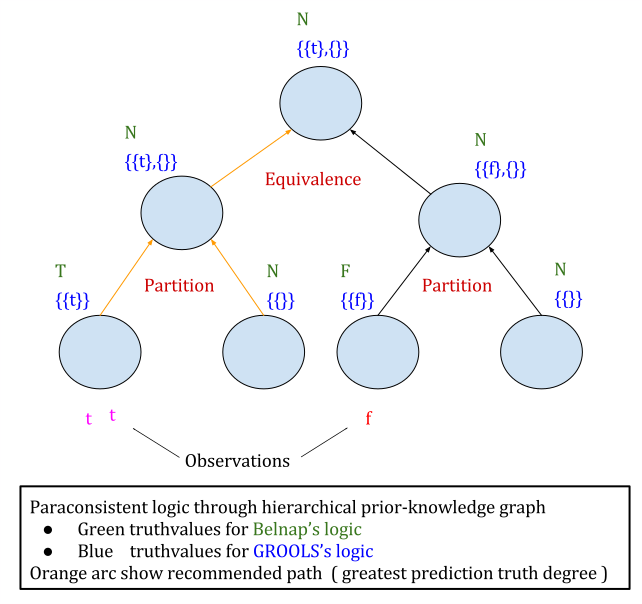
\includegraphics[width=\textwidth]{img/GROOLS_vs_belnap_1.pdf}
    \caption{  }
    \label{fig:grools_belnap_1}
\end{shadedfigure}

\begin{shadedfigure}
    \centering
    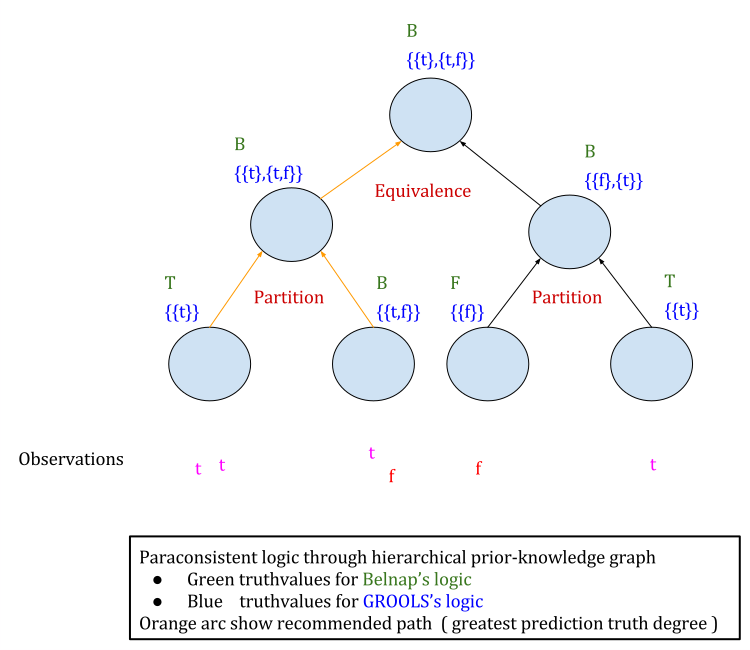
\includegraphics[width=\textwidth]{img/GROOLS_vs_belnap_2.pdf}
    \caption{  }
    \label{fig:grools_belnap_2}
\end{shadedfigure}

\subbibliography
\end{refsegment}